\documentclass{article}
\setlength{\parskip}{1em}
\usepackage{amsmath}
\usepackage{graphicx}
\graphicspath{ {./images/} }

\begin{document}

\centerline{\sc \large Reaction Wheel Stabilized Inverted Pendulum}
\vspace{.25pc}
\centerline{\sc \small optimal control, state space, and quaternions, oh my}
\vspace{.5pc}
\centerline{\sc Trent Fehl}
\vspace{1pc}

\begin{abstract}
In an attempt to develop some new skills, I started development of an 
inverted pendulum. This paper describes the system and the optimal 
controller development for the reaction wheel stabilized inverted pendulum.
Not included in this paper is the printed circuit board design, part 
selection, CAD models for the wheels, and machine paths for wheel manufacture.
I drew on papers concerning optimal control of a cart stabilized inverted 
pendulum, PID control of a reaction wheel stabilized inverted pendulum, 
and finally satellite control systems papers that utilize quaternions.
\end{abstract}

\section*{\small System Description}
This inverted pendulum is stabilized by the spinning of reaction wheels
mounted to the end of the pendulum. Only the case of a pendulum which is 
initiated and is controlled to its inverted position is being considered.
In addition to the wheels at the end of the pendulum rod, there is mass
associated with motors, a printed circuit board, batteries, and structure.
Theses are not shown in the image below but their masses are configurable 
variables for the control system.

\begin{figure}[h]
\centering
\begin{minipage}{.5\textwidth}
 \centering
 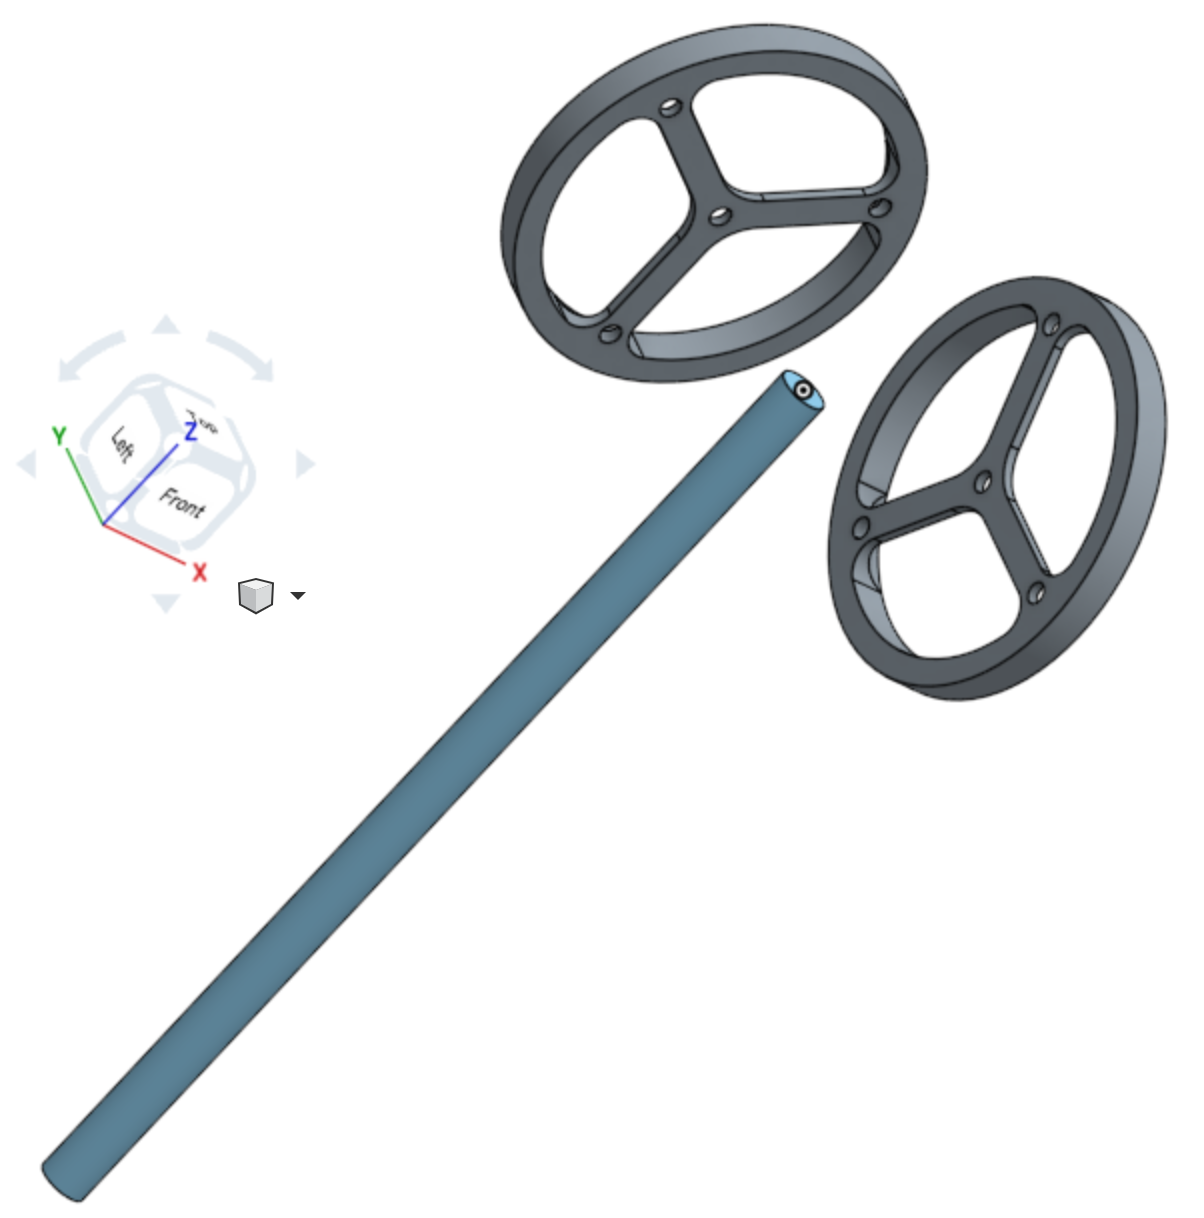
\includegraphics[width=1\linewidth]{system_angle}
 \caption{System rotated.}
\end{minipage}%
\begin{minipage}{.5\textwidth}
 \centering
 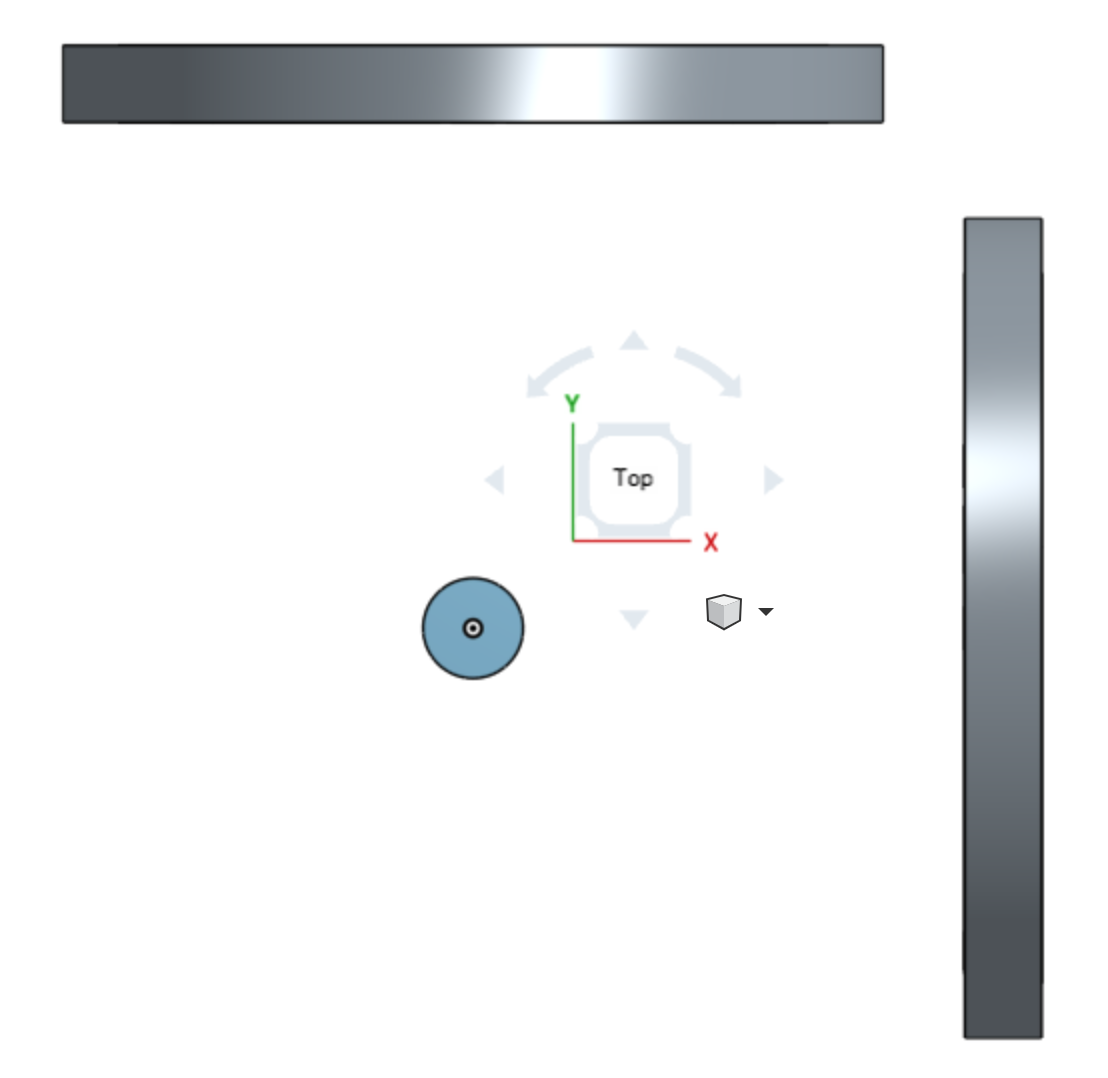
\includegraphics[width=1\linewidth]{system_top}
 \caption{Top of system.}
\end{minipage}
\end{figure}

The equations of motion were determined and are described below.
These equations are used to build a state space representation
of the system. The state space representation takes the form 
$\boldsymbol{\dot{x}(t)} = \boldsymbol{A}\boldsymbol{x(t)} + 
\boldsymbol{B}\boldsymbol{u(t)}$ where $x(t)$ is the system state 
at time $t$, $u(t)$ is the input to the system at time $t$, and $A$ 
and $B$ are their respective coefficients which are described by 
the equations below. See \cite{mitstatespace} for more information 
about this representation. Below is the first set of equations.

$$\dot{q}_1 = \omega_x,\;  
\dot{q}_2 = \omega_y,\;
\dot{q}_3 = \omega_z$$

Using small angle approximation as used in (reference) the rate of 
change of each quaternion is approximately equal to the pendulum 
$\omega$, rotational speed, for the respective axis. The quaternion
representation used in this paper is $\boldsymbol{q} = q_0 + q_1\,i 
+ q_2\,j + q_3\,k$. $\boldsymbol{q}$ and $\boldsymbol{w}$ are measured 
by a 3-axis accelerometer and a 3-axis gyroscope, respectively.

$$\dot{\omega}\; =\;
\frac{-b_\omega}{I_\omega + I}\,\omega_\omega\;
+ \frac{b_r}{I_\omega + I}\,\omega_r\;
+ \frac{glm}{I_\omega + I}\,2q\;
+ \frac{k_s}{I_\omega + I}\,\mu$$

Above describes the rate of change of the rotational speed of the 
pendulum, or the angular acceleration. Where:
\begin{itemize}
\setlength{\itemindent}{.5in}
\item $-b_w$ is the friction in the wheel bearings.
\item $\omega_w$ is rotational speed of the wheel.
\item $I_w$ is the moment of inertia of the wheel.
\item $I$ is the moment of inertia of the system.
\item $b_r$ is the friction in the rotation of the pendulum rod.
\item $\omega_r$ is the rotational speed of the pendulum rod.
\item $g$ is gravitational acceleration (-9.81 $m/s^2$).
\item $l$ is the length of the pendulum rod.
\item $m$ is the combined mass at the end of the pendulum rod.
\item $k_s$ is ?
\end{itemize}

$$\dot{\omega}_\omega\; =\;
\frac{-b_\omega}{I_\omega}\,\omega_\omega\;
+ \frac{k_s}{I_\omega}\,\mu$$

Using the equations of motion, the state space represenation takes
the following form:
\[
\begin{bmatrix}
\underset{3\times 1}{\boldsymbol{\dot{q}}} \\
\underset{3\times 1}{\boldsymbol{\dot{\omega}_p}} \\
\underset{3\times 1}{\boldsymbol{\dot{\omega}_w}}
\end{bmatrix}
=
\begin{bmatrix}
\underset{3\times 3}{\boldsymbol{0}} & \underset{3\times 3}{\boldsymbol{A_{12}}} & \underset{3\times 3}{\boldsymbol{0}} \\
\underset{3\times 3}{\boldsymbol{A_{21}}} & \underset{3\times 3}{\boldsymbol{A_{22}}} & \underset{3\times 3}{\boldsymbol{A_{23}}} \\
\underset{3\times 3}{\boldsymbol{0}} & \underset{3\times 3}{\boldsymbol{0}} & \underset{3\times 3}{\boldsymbol{A_{33}}}
\end{bmatrix}
\begin{bmatrix}
\underset{3\times 1}{\boldsymbol{q}} \\
\underset{3\times 1}{\boldsymbol{\omega_p}} \\
\underset{3\times 1}{\boldsymbol{\omega_w}}
\end{bmatrix}
+
\begin{bmatrix}
\underset{3\times 3}{\boldsymbol{0}} \\
\underset{3\times 3}{\boldsymbol{A_{21}}} \\
\underset{3\times 3}{\boldsymbol{A_{31}}}
\end{bmatrix}
\begin{bmatrix}
\underset{3\times 1}{\boldsymbol{\mu}}
\end{bmatrix}
\]

\begin{thebibliography}{9}
\bibitem{mitstatespace} 
State-Space Representation of LTI Systems, Derek Rowell October 2002
\\\texttt{http://web.mit.edu/2.14/www/Handouts/StateSpace.pdf}
\end{thebibliography}

\end{document}
